\documentclass[compress]{beamer}
\usetheme{sthlm}

%-=-=-=-=-=-=-=-=-=-=-=-=-=-=-=-=-=-=-=-=-=-=-=-=
%        LOADING BEAMER PACKAGES
%-=-=-=-=-=-=-=-=-=-=-=-=-=-=-=-=-=-=-=-=-=-=-=-=

\usepackage{
booktabs,
datetime,
dtk-logos,
graphicx,
multicol,
pgfplots,
ragged2e,
tabularx,
tikz,
wasysym,
multirow,
float,
caption,
subcaption
}

\definecolor{mygreen}{RGB}{113, 166, 70}
\definecolor{myblue}{RGB}{68, 140, 185}
\definecolor{myred}{RGB}{217, 98, 55}
\definecolor{mypurple}{RGB}{83, 65, 126}
\definecolor{solviaveis}{RGB}{188, 207, 241}

\pgfplotsset{compat=1.8}

\usepackage[utf8]{inputenc}
\usepackage[portuguese]{babel}
\usepackage[T1]{fontenc}
\usepackage{newpxtext,newpxmath}
\usepackage{listings}

\lstset{ %
language=[LaTeX]TeX,
basicstyle=\normalsize\ttfamily,
keywordstyle=,
numbers=left,
numberstyle=\tiny\ttfamily,
stepnumber=1,
showspaces=false,
showstringspaces=false,
showtabs=false,
breaklines=true,
frame=tb,
framerule=0.5pt,
tabsize=4,
framexleftmargin=0.5em,
framexrightmargin=0.5em,
xleftmargin=0.5em,
xrightmargin=0.5em
}



%-=-=-=-=-=-=-=-=-=-=-=-=-=-=-=-=-=-=-=-=-=-=-=-=
%        LOADING TIKZ LIBRARIES
%-=-=-=-=-=-=-=-=-=-=-=-=-=-=-=-=-=-=-=-=-=-=-=-=

\usetikzlibrary{
backgrounds,
mindmap
}

%-=-=-=-=-=-=-=-=-=-=-=-=-=-=-=-=-=-=-=-=-=-=-=-=
%        BEAMER OPTIONS
%-=-=-=-=-=-=-=-=-=-=-=-=-=-=-=-=-=-=-=-=-=-=-=-=

\setbeameroption{show notes}

%-=-=-=-=-=-=-=-=-=-=-=-=-=-=-=-=-=-=-=-=-=-=-=-=
%        BEAMER COMMANDS
%-=-=-=-=-=-=-=-=-=-=-=-=-=-=-=-=-=-=-=-=-=-=-=-=


%-=-=-=-=-=-=-=-=-=-=-=-=-=-=-=-=-=-=-=-=-=-=-=-=
%
%	PRESENTATION INFORMATION
%
%-=-=-=-=-=-=-=-=-=-=-=-=-=-=-=-=-=-=-=-=-=-=-=-=

\title{Otimização Linear}
\subtitle{DCE692 - Pesquisa Operacional}
%\date{\small{\jobname}}
\author{\texttt{Iago Carvalho}}
\institute{\texttt{Departamento de Ciência da Computação}}

\hypersetup{
pdfauthor = {Iago A. Carvalho},      
pdfsubject = {Pesquisa Operacional},
pdfkeywords = {},  
pdfmoddate= {D:\pdfdate},          
pdfcreator = {WriteLaTeX}
}

\begin{document}

\begin{frame}
\titlepage

\end{frame}

%% --------------------------------------------------------

\begin{frame}{Otimização Linear}

Apesar deste curso ser sobre Pesquisa Operacional, nós vamos nos concentrar em tópicos de Otimização Linear

\vspace{0.5cm}

O objetivo da otimização linear é resolver modelos matemáticos lineares
\begin{itemize}
    \item Sistema de equações lineares
    \item Uma (ou mais) funções objetivo
    \item Conjunto de restrições
    \item Variáveis no domínio dos reais ($\mathbb{R}$)
\end{itemize}

\vspace{0.5cm}

Deve-se atribuir um valor para cada uma das variáveis do problema de tal forma que
\begin{itemize}
    \item A função objetivo seja minimizada (ou maximizada)
    \item Todas as restrições sejam respeitadas
\end{itemize}
\end{frame}

%% --------------------------------------------------------

\begin{frame}{Programação Linear}

\begin{columns}[T]
    \begin{column}{.3\textwidth}
        \vspace{1.8cm}
        $\begin{matrix}
        \min & 2x + y\\ 
             & x + y & \leq 6 \\ 
             & x - y & \geq 4 \\ 
             & x & \geq 0\\ 
             & y & \geq 0
        \end{matrix}    
        $
    \end{column}
    \begin{column}{.68\textwidth}
        \centering 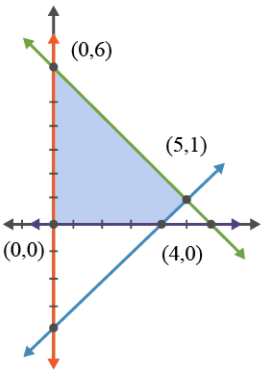
\includegraphics[width=0.6\textwidth]{images/modelo_pl.png}
    \end{column}
\end{columns}

\end{frame}

%% --------------------------------------------------------

\begin{frame}{Otimização Linear}

O principal uso de modelos de programação linear é para otimizar (encontrar o mínimo ou o máximo) de algo
\begin{itemize}
    \item Maximizar o lucro
    \item Minimizar as perdas
    \item Minimizar o tempo gasto
    \item Minimizar número de funcionários
    \item Maximizar o número de produtos produzidos
    \item Minimizar gasto de combustível
    \item $\ldots$
\end{itemize}
\end{frame}

%% --------------------------------------------------------

\begin{frame}{Otimização Linear}

Modelos de otimização linear normalmente tentam representar um problema de mundo real através de um sistema de equações

A \textbf{função objetivo} representa aquilo que você quer otimizar
\begin{itemize}
    \item Minimizar ou maximizar
\end{itemize}

As \textbf{variáveis} representam a tomada de decisão

\begin{itemize}
    \item Vou utilizar esta rota ou aquela?
    \item Quantos produtos deste tipo eu vou produzir?
\end{itemize}

As \textbf{restrições} representam as limitações existentes

\begin{itemize}
    \item Qual é o número máximo de horas por dia que estes funcionários podem trabalhar?
    \item Quantos metros cúbicos de madeira eu tenho para produzir estes móveis?
    \item Quantos caminhões eu possuo para fazer entregas?
\end{itemize}

\end{frame}

%% --------------------------------------------------------

\begin{frame}{Otimização Linear}

\begin{columns}[T]
    \begin{column}{.45\textwidth}
        \vspace{1.8cm}
        $\begin{matrix}
        \textcolor{blue}{\min} & \textcolor{blue}{2x + y}\\ 
             & \textcolor{red}{x + y} & \textcolor{red}{\leq 6} \\ 
             & \textcolor{red}{x - y} & \textcolor{red}{\geq 4} \\ 
             & \textcolor{red}{x} & \textcolor{red}{\geq 0}\\ 
             & \textcolor{red}{y} & \textcolor{red}{\geq 0}
        \end{matrix}    
        $
    \end{column}
    \begin{column}{.43\textwidth}
        \vspace{1.8cm}
        \textcolor{blue}{Função objetivo} \\
        \textcolor{red}{Restrições}
    \end{column}
\end{columns}

\end{frame}

%% --------------------------------------------------------

\begin{frame}{Otimização Linear}

\begin{columns}[T]
    \begin{column}{.45\textwidth}
        \vspace{1.8cm}
        $\begin{matrix}
        \textcolor{magenta}{\min} & \textcolor{blue}{2\textbf{x} + \textbf{y}}\\ 
             & \textcolor{red}{\textbf{x} + \textbf{y}} & \textcolor{red}{\leq 6} \\ 
             & \textcolor{red}{\textbf{x} - \textbf{y}} & \textcolor{red}{\geq 4} \\ 
             & \textcolor{cyan}{\textbf{x}} & \textcolor{cyan}{\geq 0}\\ 
             & \textcolor{cyan}{\textbf{y}} & \textcolor{cyan}{\geq 0}
        \end{matrix}    
        $
    \end{column}
    \begin{column}{.43\textwidth}
        \vspace{1.8cm}
        \textcolor{magenta}{Direção da função objetivo} \\
        \textcolor{blue}{Função objetivo} \\
        \textcolor{red}{Restrições} \\
        \textbf{Variáveis (em negrito)} \\
        \textcolor{cyan}{Restrições de domínio das variáveis}
    \end{column}
\end{columns}

\end{frame}

%% --------------------------------------------------------

\begin{frame}{Otimização Linear}

\begin{columns}[T]
    \begin{column}{.58\textwidth}
        \centering 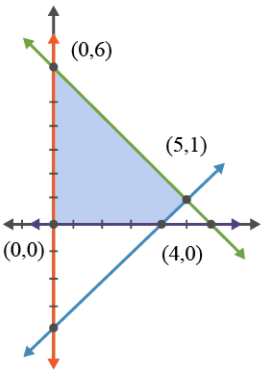
\includegraphics[width=0.9\textwidth]{images/modelo_pl.png}
    \end{column}
    \begin{column}{.4\textwidth}
        \vspace{1.8cm}
        \textcolor{mygreen}{$x + y \leq 6$} \\
        \vspace{0.25cm}
        \textcolor{myblue}{$x - y \geq 4$} \\
        \vspace{0.25cm}
        \quad~~~\textcolor{myred}{$y > 0$} \\
        \vspace{0.25cm}
        \quad~~~\textcolor{mypurple}{$x > 0$} \\
        \vspace{0.25cm}
        \textcolor{solviaveis}{\textbf{Soluções viáveis}}
    \end{column}
\end{columns}

\end{frame}

%% --------------------------------------------------------

\begin{frame}{Otimização Linear}

\begin{columns}[T]
    \begin{column}{.58\textwidth}
        \centering 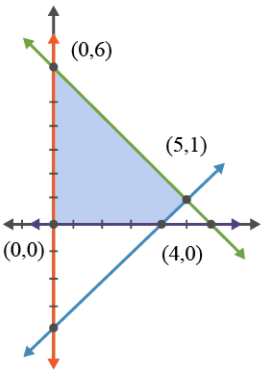
\includegraphics[width=0.9\textwidth]{images/modelo_pl.png}
    \end{column}
    \begin{column}{.4\textwidth}
        \vspace{1cm}
        O espaço azul representa o conjunto de soluções viáveis de nosso problema
        \begin{itemize}
            \item Soluções ótimas
            \item Soluções sub-ótimas
        \end{itemize}
        
        \vspace{1cm}
        
        Solução ótima está em um vértice
        \begin{itemize}
            \item Encontro de duas ou mais restrições
        \end{itemize}
    \end{column}
\end{columns}

\end{frame}

%% --------------------------------------------------------

\begin{frame}{Otimização Linear}

\begin{columns}[T]
    \begin{column}{.58\textwidth}
        \centering 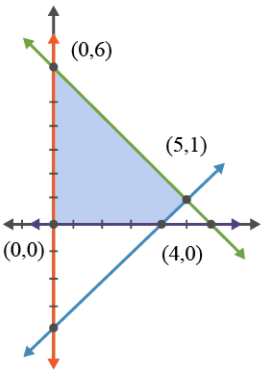
\includegraphics[width=0.9\textwidth]{images/modelo_pl.png}
    \end{column}
    \begin{column}{.4\textwidth}
        \vspace{2cm}
        \qquad~~~~$\min~~2x + y$
        \vspace{0.2cm}
        \begin{table}[]
            \centering
            \begin{tabular}{@{}ccc@{}}
            \toprule
            \textbf{x} & \textbf{y} & \textbf{resultado} \\ \midrule
            0          & 0          & 0     \\
            0          & 6          & 6     \\
            5          & 1          & 11    \\
            4          & 0          & 8     \\ \bottomrule
            \end{tabular}%
        \end{table}
    \end{column}
\end{columns}

\end{frame}

\end{document}